% TODO revisar comas
% TODO Schema
\chapter{Solución propuesta}

    En este cápitulo, comentaremos la solución que hemos propuesto, y que
    hemos llevado a cabo para conseguir una autenticación a través de la
    federación de identidad para SSH.

    \section{Posibles soluciones barajadas}

    La parte más importante de este proyecto es la conexión entre la
    federación de identidad, basada en aplicaciones web, y los servidores
    SSH.

    Para conseguir esta conexión, es casi imprescindible una pequeña
    aplicación web, que esté tras un proveedor de servicio, y la cual pueda
    acceder a los atributos del usuario, una vez este se haya autenticado
    en el IdP de su organización.

    Esta aplicación web, será la que diga si un usuario está
    autenticado en la federación o no, y su funcionamiento variará
    ligeramente, según la implementación concreta de la solución.

    \textbf{Servidor ssh}:

    Como primera opción se barajó la idea de utilizar un modulo PAM
    (Plugable Authentication Method), ya que el servidor SSH permite este
    tipo de autenticación. Los módulos PAM son un método que permite al
    administrador controlar cómo se realiza el proceso de autenticación de
    los usuario para aplicaciones, a través de unas bibliotecas.

    La opción de los módulos PAM permitiría el acceso sin tener que tocar
    el servidor SSH, sino simplemente añadiendo un módulo al sistema, y
    cambiando una línea en un fichero de configuración.

    Pero como inconveniente tiene que estos módulos autentican con usuario
    y contraseña, por lo que o se le pasa el usuario y contraseña al
    servidor SSH (cosa que no queremos), o se crea una cuenta de un solo
    uso.

    Otra posible solución es utilizar el método de autenticación por clave
    pública que proporciona el servidor openssh. Este método permite
    autenticar a un usuario sin que este tenga que introducir su
    contraseña, y sería lo más automático posible.

    Este método funciona buscando la clave pública del usuario en un
    fichero del sistema local. Pero nosotros no tenemos un fichero en cada
    servidor SSH con las claves de los usuarios autenticados. Además esta
    lista de usuarios será dinámica.

    La solución que hemos elegido para solventar el problema es la segunda,
    pero es necesario que además de mirar en los ficheros locales, pregunte
    a un servidor intermedio, para saber qué usuarios están autenticados en
    la federación. Para esto es necesario tocar un poco el código del
    servidor SSH, sin cambiar su funcionamiento normal, pero añadiendo la
    opción de pedir claves públicas a un servidor externo.

    Como hemos optado por la opción de pedir la clave pública del usuario
    desde el servidor SSH a un servido externo, se nos presenta un abanico
    de posibilidades para guardar las claves.

    \begin{itemize}
    
    \item Fichero
    \item Base de datos
    \item Directorio

    \end{itemize}

    En nuestro caso hemos optado por utilizar un directorio, puesto que la
    federación de identidad está muy ligada al uso de esta tecnología para
    almacenamiento de usuarios, y lo que vamos a almacenar es un conjunto
    de usuarios y sus claves públicas para que el servidor SSH pueda
    acceder a ellas.

    \section{Solución elegida}

    %TODO considerar repetir la figura
    La solución propuesta consta de varias partes, como se puede apreciar
    en la figura \ref{fig:casodeuso}. Las partes que incumben a este
    proyecto son:

    \begin{itemize}
        
        \item La aplicación web protegida tras el SP global de la
        federación. Esta aplicación será la encargada de verificar que el
        usuario se ha autenticado en la federación, y hará las operaciones
        pertinentes para que se pueda acceder a los datos necesarios del
        usuario a través de un medio que no sea un navegador web, de tal
        forma que el servidor SSH pueda autenticar.

        \item El servidor de claves. Será un servidor que se encargará de
        almacenar los datos de los usuarios autenticados en la federación,
        para facilitar el acceso a los mismos por parte del servidor SSH.
        Este servidor será el punto intermedio que enlace la federación
        (web) con el servicio de SSH.

        \item Los servidores SSH. Todos los servidores que presten el
        servicio de SSH sobre federación de identidad, deberán autenticar a
        los usuarios en la federación de alguna otra forma. Para
        conseguir esto está el servidor de claves, que facilitará la
        comunicación entre la federación y los servidores.

    \end{itemize}

    \section{Parche para openssh (proceso de autenticación sshd)}
    \label{openssh}

    Para implementar la solución elegida, es necesario tocar algo del
    código del servidor de SSH de openssh, sshd.

    Una de las grandes ventajas del software libre es que si una aplicación
    no cumple los requisitos que necesitamos, pero está cerca de
    conseguirlo, siempre se puede coger el código del proyecto, estudiarlo,
    y si es viable, mejorarlo o adaptarlo para que pueda cumplir nuestras
    necesidades.

    En nuestro caso, el servidor SSH hace casi todo lo que queremos que
    haga. Pero no autentica frente a una federación. Una posible solución
    sería implementar un servidor SSH que sí hiciera la autenticación de
    esta manera, pero sería tremendamente costoso. Por esta razón es mucho
    más simple el basarse en un proyecto maduro, como es openssh, y
    modificarlo de tal forma que se adapte a nuestras necesidades.

    Gracias a la licencia libre del proyecto openssh, BSD License, es
    posible acceder a todo el código, se puede estudiar, modificar, y
    distribuir de forma libre, por lo que nuestro proyecto es viable.

    Por lo tanto nos hemos basado en este proyecto, cogiendo su código y
    desarrollando un parche que permita la autenticación a través de
    certificado de clave pública, pero situado este certificado en un
    servidor de claves, en lugar de en un fichero local del sistema.

    La autenticación del servidor SSH funciona de la siguiente manera:

    \begin{enumerate}

    \item Intenta la autenticación por certificado de clave pública. Busca
    en el fichero \$HOME/authorized\_keys, y prueba que el usuario que está
    intentando autenticarse tiene la clave privada de alguna de las claves
    que aparecen en este fichero.

    \item Si no consigue autenticar, y está activa la autenticación por
    módulos PAM, el servidor pedirá una contraseña al usuario, y se
    ejecutará la pila de módulos.

    \item En otro caso, autenticará con los usuarios del sistema.

    \end{enumerate}

    En este esquema de funcionamiento, tenemos que encajar nuestro sistema
    de autenticación de identidad federada. Buscamos la mayor comodidad
    posible para el usuario, así pues, queremos que el usuario no tenga que
    introducir ninguna contraseña en el servidor SSH.

    Si llega al paso dos de la autenticación del SSH, el servidor pedirá
    automáticamente una contraseña al usuario, y dado que queremos evitar
    esta incomodidad, no es viable el crear un módulo PAM que autentique
    en la federación de identidad.

    Por esta razón es necesario tocar el código del servidor SSH. Más
    concretamente la parte de autenticación por clave pública. Ya que
    utilizaremos este sistema para identificar unívocamente al usuario que
    quiere autenticarse. Ya que no se va a introducir ninguna contraseña,
    será necesario que el usuario tenga algo que lo identifique. En el caso
    de la federación de identidad por páginas web, se utiliza una cookie
    que guarda el navegador. Para nuestro caso, la clave privada del
    usuario servirá para identificarlo, teniendo acceso el servidor SSH a
    la clave pública, una vez que el usuario esté autenticado en la
    federación.

    Por lo tanto la autenticación del servidor SSH parcheado quedaría así:

    \begin{enumerate}

    \item Intenta la autenticación por certificado de clave pública. Busca
    en el fichero \$HOME/authorized\_keys, y prueba que el usuario que está
    intentando autenticarse tiene la clave privada de alguna de las claves
    que aparecen en este fichero.

    \item \textbf{Si no consigue autenticar, pregunta al servidor de claves
    de la federación por el usuario. Si el usuario está autenticado, el
    servidor de claves le devolverá la clave pública del mismo. Con esta
    clave pública intentará autenticar al usuario, que sólo tendrá acceso
    si tiene la clave privada}

    \item Si no consigue autenticar, y está activa la autenticación por
    módulos PAM, el servidor pedirá una contraseña al usuario, y se
    ejecutará la pila de módulos.

    \item En otro caso, autenticará con los usuarios del sistema.

    \end{enumerate}

    Se puede ver el funcionamiento en el siguiente esquema
    (\ref{fig:funcionamientossh}):

    \begin{figure}[htp!]
        \centering
            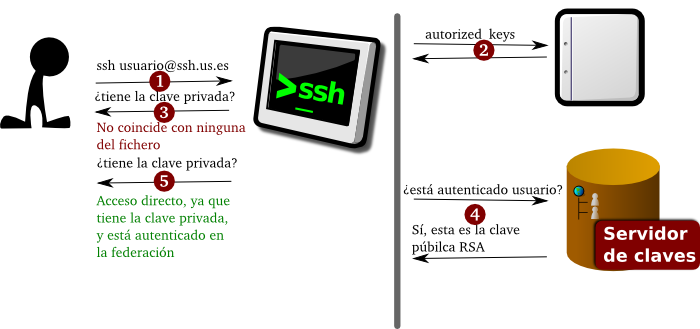
\includegraphics[width=\textwidth]{img/funcionamientossh.png}
            \caption{Funcionamiento SSH}
        \label{fig:funcionamientossh}
    \end{figure}


        \subsection{Posibles soluciones al SSO para SSH}

        Durante la realización de este proyecto han surgido algunos
        detalles y funcionalidades que se podrían implementar para el
        servidor SSH, y que se podrían utilizar de forma independiente al
        proyecto aquí descrito.

        Una de estas posibilidades, y quizás la de mayor interés, y que
        tendría entidad propia fuera de este proyecto, es el Single Sing-On
        para SSH.

        %TODO mirar comillas
        Para realizar la tarea de SSO, es necesario que el cliente
        autenticado tenga un ``token'' o algo que lo identifique
        unívocamente, en nuestro caso sería la clave privada de SSH. Y el
        servidor debería conocer quién está autenticado, en nuestro caso
        preguntando al servidor de claves.

        Para el caso de SSO únicamente, sin autenticación por federación,
        sería necesario retocar el parche del servidor SSH para que al
        acceder a un servidor a través de usuario y contraseña, este
        servidor comunicara al servidor de claves que el usuario se ha
        autenticado. Así cuando el mismo usuario vaya a acceder al mismo
        servidor, o incluso a otro dentro del SSO, tendría acceso directo.

        Este concepto lleva consigo un par de pequeños problemas, y es que
        se ha de poder acceder a alguno de los servidores introduciendo la
        clave, lo que implica que el usuario ha de tener al menos la clave
        de uno de los servidores de SSH, o por lo menos debe conocer la
        clave pública de este usuario de manera permanente.

        El otro problema es que el servidor donde se autentique el usuario
        por primera vez, ha de conocer la clave pública de este usuario
        para informar al servidor de claves de quién se ha autenticado.
        Otra alternativa sería que el servidor de claves tuviera a todos
        los usuarios en un principio registrados, pero no activos, por lo
        que decir que alguien se ha autenticado tan solo sería poner a este
        usuario como activo.
    
    \section{Servidor de claves}

    En principio la idea del servidor de claves era que fuera un servidor
    independiente, con un protocolo simple, que solo permitiera preguntar
    si un usuario está autenticado, y en caso afirmativo, ser recibiría la
    clave del mismo.

    La primera versión del protocolo simple sería:
    \begin{itemize}
    \item Peticiones al servidor:

        \begin{verbatim}

        USR:nombre
        XIT

        \end{verbatim}

        La orden USR es la petición de la clave de un usuario, y la orden
        XIT indica desconexión.

    \item Respuestas del servidor:

        El servidor responderá con la clave pública del usuario, o con la
        cadena ``NOT FOUND'', si no lo ha encontrado.

    \end{itemize}

    Esta implementación facilitaría enormemente la parte del parche al
    servidor SSH, puesto que tan solo se necesita hacer una conexión por
    socket normal, sin necesidad de utilizar ninguna librería
    complementaria.

    Por otra parte, con esta implementación de un protocolo simple sería
    muy fácil cambiar el almacenamiento de los usuarios, tan solo creando
    una interfaz que convirtiera las consultas al sistema de almacenamiento
    elegido a este protocolo. Así pues sería muy fácil almacenar los
    usuarios con ficheros de texto plano, con un sistema de base de datos
    relacional, con un servicio de directorio, etc.
    
    Sin embargo, dificulta la parte del servidor de claves, que ya tiene
    que ser una implementación propia, que utilice un almacenamiento de
    usuarios y claves determinado.

    Como esta fue la primera aproximación, se ha implementado un servidor
    de claves, de ejemplo en python. En principio almacenaba los usuarios y
    las claves en texto plano. Posteriormente se extendió para realizar el
    almacenamiento en una base de datos MySQL. Y en realidad incorporar
    nuevos sistemas de almacenamiento es algo tan simple como implementar
    una clase con un metodo \textit{get\_rsa(nombre\_de\_usuario)} que devuelva
    la clave pública RSA del usuario si está autenticado, y en otro caso
    que devuelva una cadena vacía.

    Tratando de buscar el mínimo impacto en el código del servidor SSH, las
    peticiones al servidor de claves se realizan en una función, que está
    implementada en un fichero aparte, por lo que en el código del servidor
    tan solo hay que incluir la llamada a esta función, y se puede variar
    el modo de funcionamiento de la petición. De esta forma si se varía el
    protocolo de comunicación entre el servidor SSH y el servidor de claves
    no haría falta tocar el código real del servidor SSH, solamente la
    función que es llamada desde el mismo, y que es de implementación
    propia, por lo que no afectaría al funcionamiento normal del mismo.

    Por otra parte, si el desarrollo habitual del servidor varía alguna
    parte de la autenticación, el parche es fácilmente adaptable a futuras
    versiones, puesto que del código original toca lo menos posible.

    Tras esta primera implementación de prueba, y tras ver que todo era
    correcto, y que funcionaba bien, decidimos incrementar la seguridad
    entre las comunicaciones.

    En un principio se optó por incrementar la seguridad del servidor de
    claves utilizando sockets ssl, pero tras observar que esto complicaría
    la solución de manera drástica, se optó por utilizar algo más simple.

    Así pues se pensó en utilizar como servidor de claves un servicio de
    directorio, y utilizar como protocolo de comunicaciones el propio
    protocolo LDAP, que tiene una versión segura.

    La opción de elegir un servicio de directorio no es algo casual, sino
    que se eligió este sistema porque cumple los requisitos necesarios para
    el servidor de claves, tal y como está definido, y además cuando se
    habla de federación de identidad, es casi imposible no hablar de
    servicios de directorio. Hoy en día la federación de identidad está muy
    ligada a este tipo de almacenamiento de usuarios, por lo tanto es una
    buena opción.

    Al utilizar un servicio de directorio como servidor de claves públicas,
    se simplifica la parte del servidor de claves, puesto que ya está
    hecho, y es muy fácil desplegar uno. Pero por otra parte se complica un
    poco la modificación al servidor SSH.

    Puesto que estamos usando el servidor SSH que viene con la
    implementación openssh, y este está en C, nuestro parche deberá hacer
    peticiones a un servidor de claves a través del protocolo de
    comunicación LDAP, desde el lenguaje C.

    Por suerte las consultas al servicio de directorio desde C no son nada
    complicadas, e implementando una simple función es posible modificar el
    parche para que el servidor SSH ahora se comunique con un servidor de
    claves a través de LDAP.

    \subsection{Esquemas LDAP}

    % TODO campos son atributos
    % entradas son objetos
    Los sistemas de directorio utilizan diferentes atributos para guardar los
    datos pertenecientes a las diferentes entradas. Cada posible campo a
    utilizar está definido en un ``Schema LDAP'', y se podrá utilizar
    siempre que la entrada tenga el ``objectclass'' que define ese campo.

    Existen muchos estándares de schemas LDAP, que suelen venir por defecto
    en la mayoría de los servicios de directorio. Y cada schema tiene sus
    atributos destinados cada uno a almacenar un tipo de dato concreto.

    Es posible utilizar un campo cualquiera, siempre que sea del mismo
    tipo, para guardar cualquier información, pero esto no es recomendable,
    puesto que esto complica la compresión de futuros usuarios y
    administradores, dado que cada campo tiene una definición de para qué
    se usa.

    Por ejemplo se puede usar el campo ``mail'' para guardar el dni del
    usuario. Pero no es correcto, ya que el campo mail está especificado
    para almacenar la dirección de correo.

    Así pues, hay que definir, o buscar unos Schemas que definan, los
    campos que necesitamos para almacenar los usuarios junto a sus claves,
    en el servidor de claves.

    En principio los datos que ha de almacenar el servidor de claves para
    este proyecto son:

    \begin{itemize}

    \item \textbf{uid} del usuario autenticado en la federación.
    \item \textbf{clave pública} del usuario autenticado en la federación.
    \item \textbf{timeout} tiempo de vencimiento de la sesión del usuario autenticado en la federación.

    \end{itemize}

    El primer campo, \textbf{uid}, está cubierto en los schemas que vienen
    por defecto, en el schema \textbf{person}.

    Para el segundo campo, en principio se pensó en utilizar el campo
    usercertificate, pero no es el más adecuado, ya que está pensado para
    almacenar un certificado personal. Así pues buscando alternativas se ha
    decidido utilizar el schema \textit{openssh-lpk}
    \url{http://dev.inversepath.com/openssh-lpk} que ofrece un atributo
    sshPublicKey, destinado para este propósito.

    Y por último, para cubrir las necesidades del segundo campo se ha
    optado por utilizar el schema \textit{schac}
    \url{http://www.terena.org/activities/tf-emc2/schac.html}, y utilizar
    el atributo schacUserStatus para guardar el timeout con el siguiente
    formato: \texttt{schac:userStatus:us.es:timeout:1205274586}, donde el
    número representa la fecha, en segundos, de expiración.

    Por supuesto se pueden utilizar otros atributos para almacenar los
    datos de usuario, y tan solo habría que cambiar la configuración del
    servidor sshd. No sería necesario recompilar el parche.

    \section{Aplicación de login}
    \label{login}
    

    La aplicación de login es también una parte importante de este
    proyecto, ya que será lo que conecte la federación con el servidor de
    claves al que consultarán los servidores SSH. Por lo tanto todo usuario
    que quiera utilizar el servicio de SSH federado deberá entrar antes en
    esta aplicación federada, para que la propia aplicación pueda tener
    acceso a los datos que le facilite el IdP del usuario en concreto, y
    así indicar al servidor de claves que el usuario está autenticado, y
    cuál es su clave pública.

    Esta aplicación, como se ha comentado anteriormente, deberá ir
    protegida tras un SP, no necesariamente perteneciente a una
    organización, puesto que la aplicación será única para todos los
    usuarios de todas las organizaciones implicadas en la federación.

    Se ha buscado que la interfaz de la aplicación sea lo más simple y
    clara posible. Al estar protegida tras un SP, todo usuario que
    intente acceder a esta página será redirigido al WAYF de la federación
    si no está autenticado aún. En el WAYF seleccionará su organización de
    origen, y será redirigido a la página de login de su IdP.

    Una vez que el usuario se autentique en su IdP, será redirigido a la
    aplicación de login, y en este momento, la aplicación tendrá acceso a
    los datos necesarios del usuario.

    La aplicación mirará si el campo especificado en la federación para
    almacenar la clave pública del usuario está asignado, y en caso
    afirmativo, cogerá la clave pública que viene dada en ese campo, y la
    introducirá en el servidor de claves. Se muestra al usuario una
    pantalla en la cual se especifica el nombre de usuario para acceder por
    SSH, así como la fecha y hora de caducidad de esa sesión.

    En el caso en el que no se encuentre la clave pública del usuario, se
    ofrece la posibilidad de introducirla manualmente, en un cuadro de
    texto. Este campo de texto también es de utilidad cuando un usuario no
    está en su puesto de trabajo habitual, y quiere acceder utilizando un
    par de claves temporal.

    Cuando se introduce de manera manual, la aplicación verifica que es una
    clave pública correcta, y la introduce en el servidor de claves,
    actualizando el timeout.

    %TODO comentar esto como posibilidad opcional
    Cada vez que se refresque esta página, la aplicación actualiza el
    timeout, como si el usuario acabara de acceder por primera vez.

    Esta es la apariencia de la aplicación de login:
     
    \begin{center}
        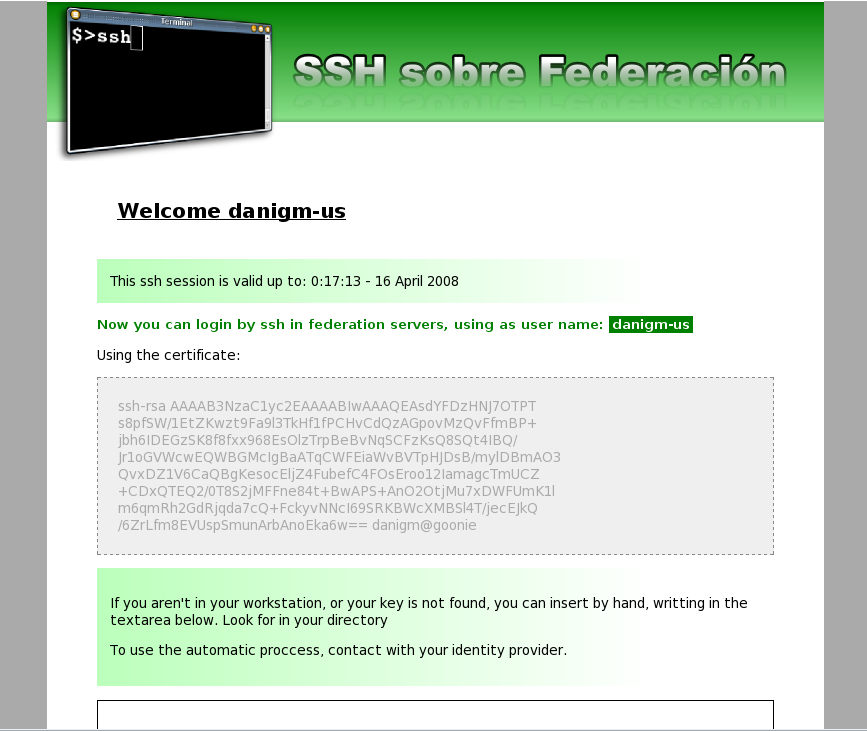
\includegraphics[width=\textwidth]{img/sshApp.png}
    \end{center}
     
    Por facilidad de desarrollo, e integración con distintos servidores
    web, se ha elegido utilizar la tecnología PHP para el desarrollo de
    esta aplicación.

    La aplicación está separada en un frontend y un backend. El frontend se
    encarga de mostrar los datos, y en el backend están definidas las
    funciones tanto de búsqueda y petición de datos, como las de
    almacenamiento en el servidor de claves.

    La implementación actual de esta aplicación está ligeramente ligada al
    SP de shibboleth 1.3. Pero es fácilmente modificable para que utilice
    otro tipo de SP, solo cambiando unas variables en el código, de tal
    forma que consulte otro tipo de cabeceras.

    Puesto que hemos decidido utilizar un servidor de claves basado en un
    servicio de directorio se han tenido que utilizar las bibliotecas
    pertinentes del lenguaje PHP para LDAP.

    Toda la información sobre atributos a consultar, y atributos necesarios
    para guardar la información está especificada en forma de variables,
    para que su modificación sea fácil.

    Para aumentar el grado de seguridad del sistema, cabe la posibilidad de
    extender la aplicación de manera sencilla, de tal forma que antes de
    almacenar los datos del usuario en el servidor de claves, informara al
    usuario sobre los datos que se van a almacenar, y pidiera confirmación.

    \section{Ejemplo aplicación creación de cuentas}

    Un problema que hay que tener en cuenta en el despliegue de este
    proyecto, es la necesidad de crear las cuentas de los usuarios de forma
    dinámica en los servidores parcheados.

    En principio, y según la implementación actual del proyecto, el
    servidor SSH parcheado supone que la cuenta de usuario existe, y por
    tanto cuando pida la clave pública al servidor de claves, generará un
    fichero temporal con esa clave en el directorio HOME de ese usuario, y
    utilizará ese fichero para hacer la autenticación por clave pública.

    Dado que esta implementación delega el problema de la creación de
    cuentas al administrador del sistema, es necesario que se creen y se
    destruyan las cuentas de manera dinámica, en el servidor.

    La delegación de la creación de cuentas en el administrador del
    sistema, permite un mayor control sobre quién va a poder acceder a este
    servicio, permitiendo crear políticas de creación de cuentas, y no
    permitiendo entrar al servidor a cualquier usuario autenticado en la
    federación.

    Para facilitar el trabajo de administración de estos servidores, y
    además ofrecer al usuario un punto central de acceso a servidores SSH,
    se ha desarrollado un ejemplo sencillo de aplicación de creación de
    cuentas.

    La idea consiste en hacer una aplicación con un aspecto visual similar
    a la de autenticación, y que ofrezca una lista de los servidores de SSH
    disponibles, junto con una corta descripción del servicio. Además da la
    posibilidad de solicitar las cuentas a los diferentes servidores, para
    así tener una creación de cuentas automática, y que no haya que hacer
    una creación de cuentas manual.

    La aplicación iría protegida tras un SP y tampoco tiene que ser parte
    de ninguna organización, al igual que la aplicación de acceso. Cuando
    el usuario acceda a la aplicación, si no está autenticado ya en la
    federación, será redirigido al WAYF. En el WAYF seleccionará su
    institución de origen, y será redirigido al IdP correspondiente, donde
    se autenticará. Una vez autenticado tendrá acceso a la aplicación, y la
    misma aplicación a partir del uid del usuario consulta si el usuario
    tiene cuenta en el servidor, y permite la creación de la cuenta, con un
    enlace.

    Para crear las cuentas desde el servidor donde esté instalada esta
    aplicación web, hay que permitir el acceso por SSH al comando useradd,
    puesto que se va a utilizar una llamada al sistema para lanzar el
    comando a través de este protocolo, y así crear la cuenta solicitada.
    Para ello, se ha introducido la clave pública de acceso SSH del
    servidor web en el fichero authorized\_keys de cada servidor SSH.

    Este despliegue tiene fallos de seguridad, puesto que cualquiera que
    tenga acceso al servidor web, tendrá acceso a la creación de cuentas de
    todos los servidores SSH.

    Una mejora de esta aplicación, y el siguiente paso lógico si esto se
    quiere implantar en un sistema federado en producción, sería utilizar
    servicios web, o llamadas a otro tipo de procesos remotos, que
    verificaran el origen de la petición, con algún sistema
    criptográficamente seguro, y tan sólo permitiendo la creación de la
    cuenta, es decir, un proceso en cada servidor, que recibiera peticiones
    del servidor web que aloja esta aplicación, y que creara las cuentas.

    El desarrollo de este sistema permitiría también definir políticas de
    creación de cuentas, dando la posibilidad de que cada administrador de
    cada servidor SSH federado definiera su política. Así por ejemplo para
    un servidor general, de poca trascendencia, se podría dejar que se
    crearan las cuentas de forma automática e inmediata, y en otro tipo de
    servidores, con recursos más limitados, se mandará un correo al
    administrador para que este se ponga en contacto con el solicitante y
    según el solicitante le permitiera la creación de la cuenta o no.

    Esta sería la aplicación de creación de cuentas:
     
    \begin{center}
        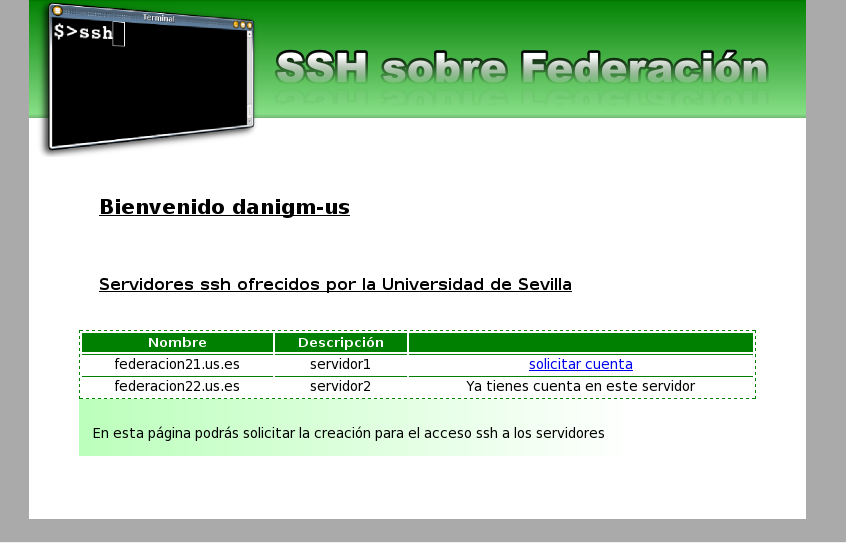
\includegraphics[width=\textwidth]{img/userAdd.png}
    \end{center}

    Otra posibilidad, menos flexible, pero más integrada sería incluir en
    el parche la posibilidad de que se crearan y destruyeran las cuentas
    de manera dinámica. Así por ejemplo, se crearía la cuenta justo antes
    de intentar autenticar al usuario.

    Esta segunda forma es mucho más invasiva en el sistema, ya que para
    implementarla el servidor SSH debe comunicarse con el sistema en
    cuestión, y hacer llamadas al mismo para crear las cuentas.

    Independientemente del sistema utilizado para la creación de las
    cuentas, la aplicación de ejemplo de creación de cuentas puede servir
    como listado de todos los servicios SSH sobre federación de identidad
    que se ofrecen. Así estaría accesible en un punto centralizado, y
    cualquier usuario de cualquier organización tendría acceso al listado y
    podría saber a qué recursos tiene acceso.
